\chapter{Anxiety}
\label{applications-efx_study_level}

Fixed effects explain the bias and variation of noisy measurements in terms of demographic, epidemiologic and study-specific variables.  Unlike random effects that vary by geographic unit, fixed effects have covariates that differ by study or country-year.  Frequently in meta-analysis of psychological disorders, such as anxiety, studies use different recall periods in the measurement of epidemiologic rates.  In this case, fixed effect study-level covariates explain the bias of the measurements resulting from different recall periods.

Anxiety disorders encompass several conditions characterized by prominent anxiety at a level which interferes with daily life.  Not all anxiety disorders manifest in similar ways.  While generalized anxiety disorder is typically marked by persistent worry, panic disorder is usually characterized by intense fear for discrete periods of time \cite{american_diagnostic_2000}.

Anxiety disorders do not have a consistent recall period for the measurement of epidemiological rates.  Therefore the data from meta-analysis has studies with measurements of point prevalence and period prevalence (i.e. 6-month or past year prevalence).  Due to the high remission rate for anxiety disorders, period prevalence is typically higher than point prevalence as seen in figure \ref{fig:app-anxiety data}.

    \begin{figure}[h]
        \begin{center}
            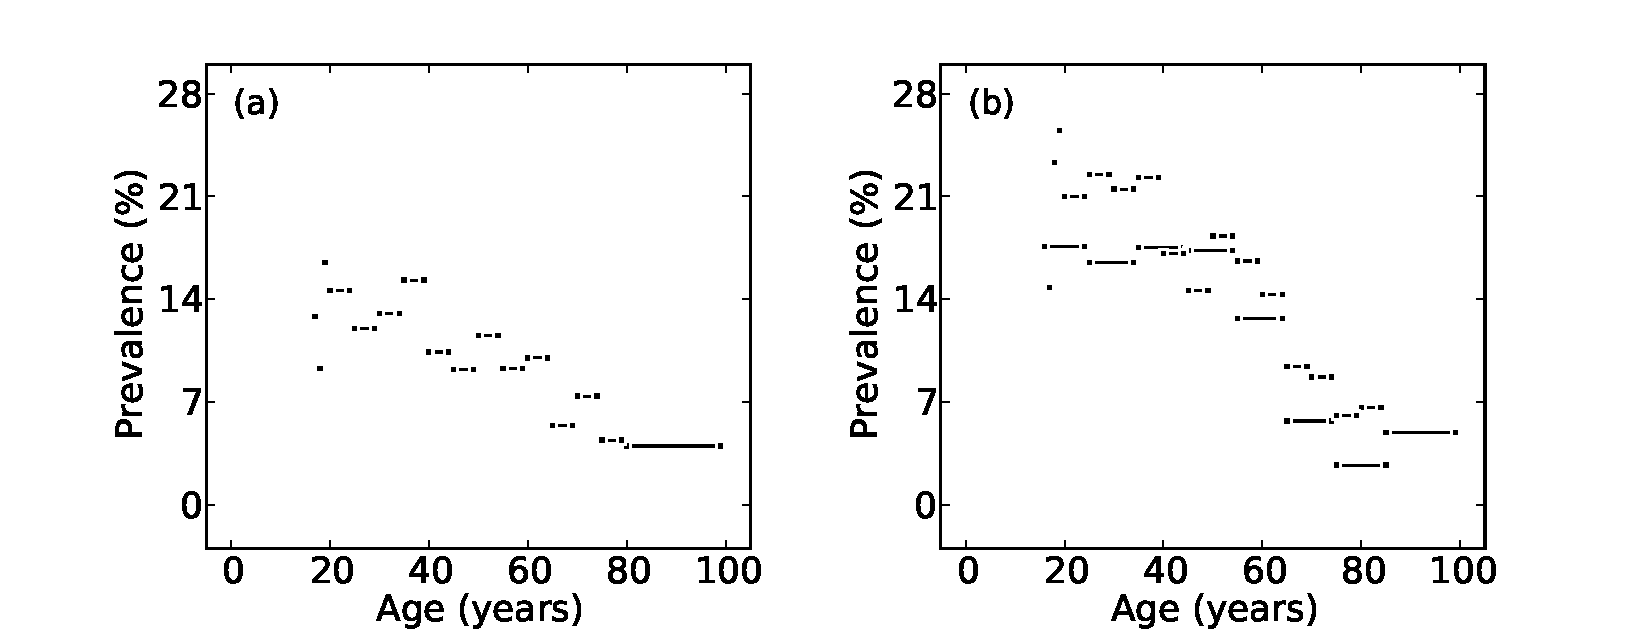
\includegraphics[width=\textwidth]{anxiety-data_by_cv.pdf}
            \caption{Data on female anxiety disorders collected in systematic review for 2000-2010 in Australasia.  Some studies measured point prevalence or period.  Period prevalence is typically higher than point prevalence because of the high remission rate for anxiety disorders.}
            \label{fig:app-anxiety data}
        \end{center}
    \end{figure}
    
Excluding period prevalence measurements reduces the quantity of data and produces results that are generally much lower than estimates using all of the data without fixed effects.  Using a fixed effect study-level covariate to explain the systematic bias and variation resulting from different recall periods lowers the prevalence estimate as seen in figure \ref{fig:app-anxiety FE}.

    \begin{figure}[h]
        \begin{center}
            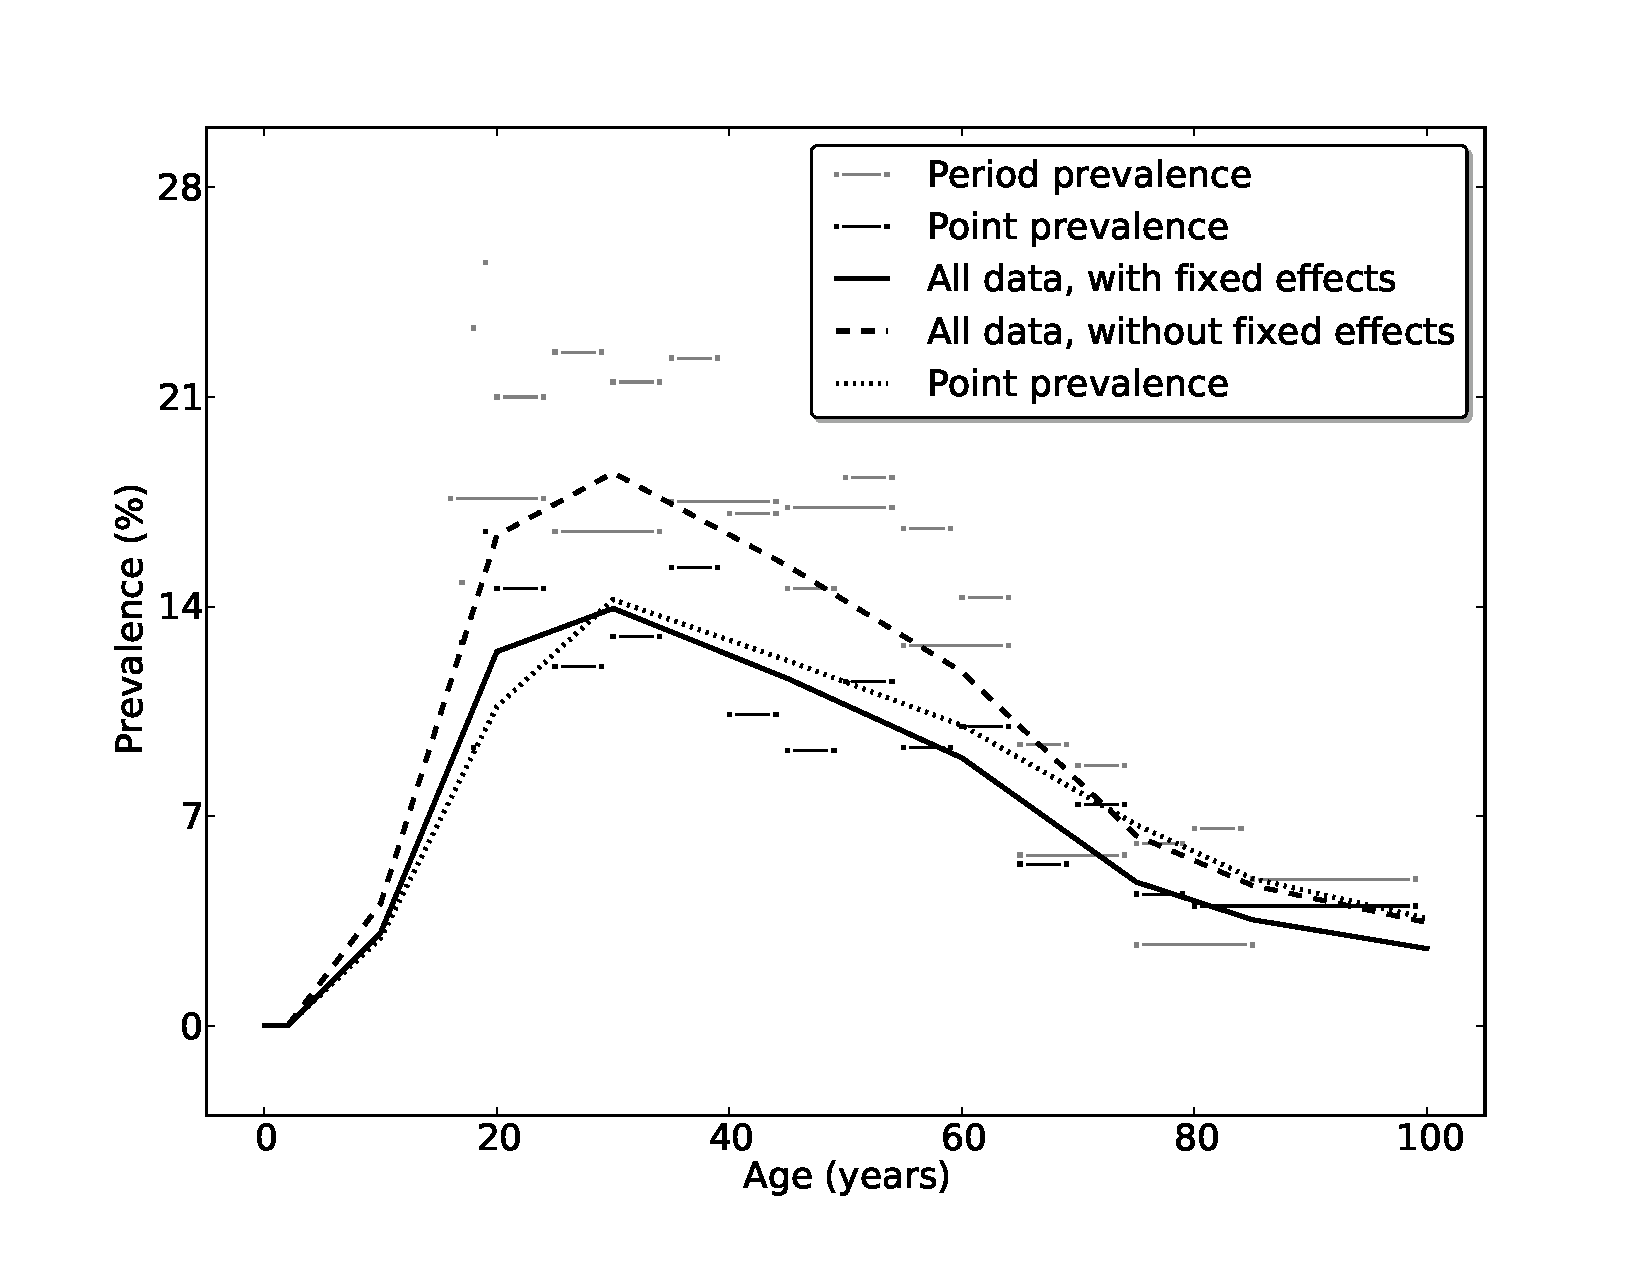
\includegraphics[width=\textwidth]{anxiety-FE.pdf}
            \caption{Prevalence estimates for anxiety disorders in 2005 for women in Australasia, with point prevalence data shown.  Notice that estimates based on all data without fixed effects are higher than point prevalence estimates.}
            \label{fig:app-anxiety FE}
        \end{center}
    \end{figure}
    
